\documentclass[11pt]{article}
% \usepackage[margin=1in]{geometry}
\usepackage[top=1in, bottom=1in, left=.5in, right=.5in]{geometry} % see geometry.pdf on how to lay out the page. There's lots.
\usepackage{amsmath,amsthm,amssymb}

% Ignore spaces in filenames
\usepackage[space]{grffile}

\usepackage[T1]{fontenc}
\usepackage{bigfoot} % to allow verbatim in footnote
\usepackage[numbered,framed]{matlab-prettifier}
\usepackage{filecontents}
\usepackage{graphicx}
\usepackage[normalem]{ulem}
\usepackage{mathtools}

\let\ph\mlplaceholder % shorter macro
\lstMakeShortInline"

\lstset{
  style              = Matlab-editor,
  basicstyle         = \mlttfamily,
  escapechar         = ",
  mlshowsectionrules = true,
}

\title{MAE 275 - Homework 6}
\author{John Karasinski}
\date{June 2, 2015}

\begin{document}
\maketitle

\section{Defining the System}
The state-space system can be defined,
\begin{equation*}
\begin{split}
\dot{\vec{x}} = A\vec{x} + B\vec{u} \\
      \vec{y} = C\vec{x} + D\vec{u}
\end{split}
\end{equation*}

\noindent where the linearized lateral aircraft equations of motion can be expressed in state space form.

$$
\vec{x}= \left[ \begin{array}{c}        v \\ p        \\ r   \\ \phi \\   \psi \end{array} \right], \qquad
\vec{u}= \left[ \begin{array}{c} \delta_a \\ \delta_r                          \end{array} \right], \qquad
\vec{y}= \left[ \begin{array}{c}        p \\ \beta                             \end{array} \right]
$$

\noindent Using the lateral equations of motion for F-89 at flight condition 8901, the resultant system is

$$
\dot{\vec{x}} = \left[ \begin{array}{ccccc}
  -8.2900e-2 &          0 & -6.6000e+2 & +3.2200e+1 &          0 \\
  -6.8939e-3 & -1.7000e+0 & +1.7200e-1 &          0 &          0 \\
  +5.1212e-3 & -6.5400e-2 & -8.9300e-2 &          0 &          0 \\
           0 &         +1 &          0 &          0 &          0 \\
           0 &          0 &         +1 &          0 &          0 \end{array} \right]
\vec{x} + \left[\begin{array}{ccc}
           0 & +7.6500e+0 \\
  +2.7300e+1 & +5.7600e-1 \\
  +3.9300e-1 & -1.3600e+0 \\
           0 &          0 \\
           0 &          0 \end{array}\right] \vec{u}
$$

$$
\vec{y} = \left[ \begin{array}{ccccc}
           0 &         +1 &           0 &           0 &           0 \\
  +1.5152e-3 &          0 &           0 &           0 &           0 \end{array} \right]
\vec{x}+\left[\begin{array}{ccc}
         0 &         0 \\
         0 &         0 \end{array}\right]\vec{u}
$$

\noindent Coupling numerators can be used to decide which loops to close in which order, and appropriate compensators can then be designed.

\clearpage
\section{Coupling Numerators}

The coupling numerators can be derived using the notes in the assignment and the HARV handout. They are

\begin{gather*}
\begin{split}
\Aboxed{\dfrac{p}{v_1} & =\dfrac{27.3 s (s^2 + 0.1747s + 3.453)} {(s+1.781) (s-0.001359) (s^2 + 0.09275s + 3.529)}} \\
\\
\dfrac{p}{v_2} & =\dfrac{0.576 s (s-2.885) (s+2.56)}
                      {(s+1.781) (s-0.001359) (s^2 + 0.09275s + 3.529)} \\
\\
\dfrac{\beta}{v_1} & =\dfrac{-0.393 (s-6.282) (s+0.04952)}
                          {(s+1.781) (s-0.001359) (s^2 + 0.09275s + 3.529)} \\
\\
\dfrac{\beta}{v_2} & =\dfrac{0.011591 (s+117.4) (s+1.753) (s-0.003733)}
                          {(s+1.781) (s-0.001359) (s^2 + 0.09275s + 3.529)} \\
\end{split}
\end{gather*}
\begin{gather*}
\begin{split}
\dfrac{p}{v_1}\biggr\rvert_{\beta \rightarrow v_2}
             & = \dfrac{27.3 s (s+118.1)}{(s+117.4) (s+1.753) (s-0.003733)} \\
\\
\Aboxed{\dfrac{\beta}{v_2}\biggr\rvert_{p \rightarrow v_1}
             & = \dfrac{0.011591 (s+118.1)}{(s^2 + 0.1747s + 3.453)}} \\
\\
\dfrac{p}{v_2}\biggr\rvert_{\beta \rightarrow v_1}
             & = \dfrac{-0.80517 s (s+118.1)}{(s-6.282) (s+0.04952)} \\
\\
\dfrac{\beta}{v_1}\biggr\rvert_{p \rightarrow v_2}
             & = \dfrac{0.54936 (s+118.1)}{(s-2.885) (s+2.56)} \\
\end{split}
\end{gather*}

\noindent From these transfer functions we can:
\begin{enumerate}
\item rule out controlling $p$ with $v_2$ first, as there is a non-minimum phase zero (s-2.885) in the transfer function that would limit the crossover frequency to values significantly below 2.885
\item rule out $\smash{\dfrac{p}{v_2}\biggr\rvert_{\beta \rightarrow v_1}}$ and $\smash{\dfrac{\beta}{v_1}\biggr\rvert_{p \rightarrow v_2}}$ due to the closed-loop unstable poles that would be produced
\end{enumerate}

\noindent This leaves only one viable option: to first close $p$ with $v_1$, then close $\beta$ with $v_2$ with the $p-v_1$ loop closed.

\clearpage
\section{Compensators}
Two compensators were designed:

\begin{gather*}
\begin{split}
GC_p &= \frac{0.18 (s+2)}{s} \\
GC_{\beta} &= \frac{3.72 (s^2 + .2s + 3.5)}{(.05 * s^2 + s)}
\end{split}
\end{gather*}

\clearpage
\begin{figure}[h!]
\begin{center}
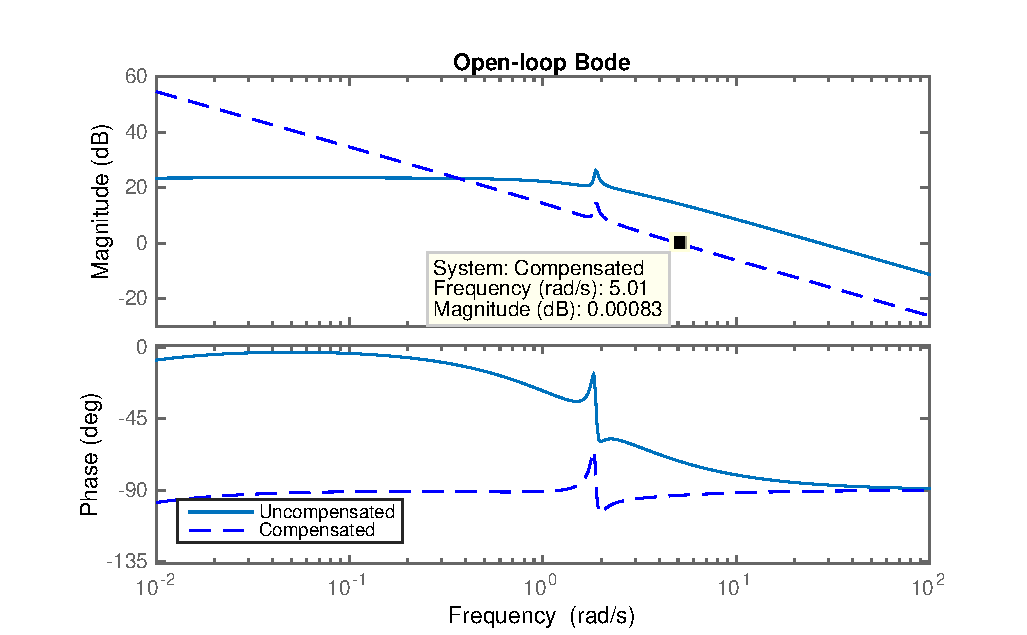
\includegraphics[height=.4\textheight]{figures/openloop_p}
\caption{Open-loop Bode Plot for $p$ loop}
\end{center}
\end{figure}

\begin{figure}[h!]
\begin{center}
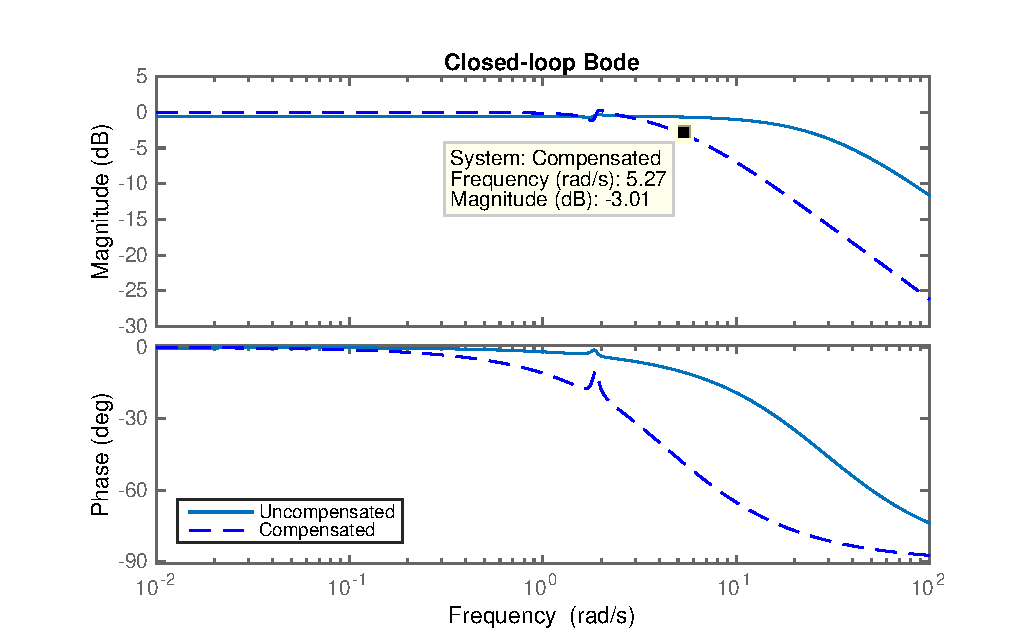
\includegraphics[height=.4\textheight]{figures/closeloop_p}
\caption{Close-loop Bode Plot for $p$ loop}
\end{center}
\end{figure}

\begin{figure}[h!]
\begin{center}
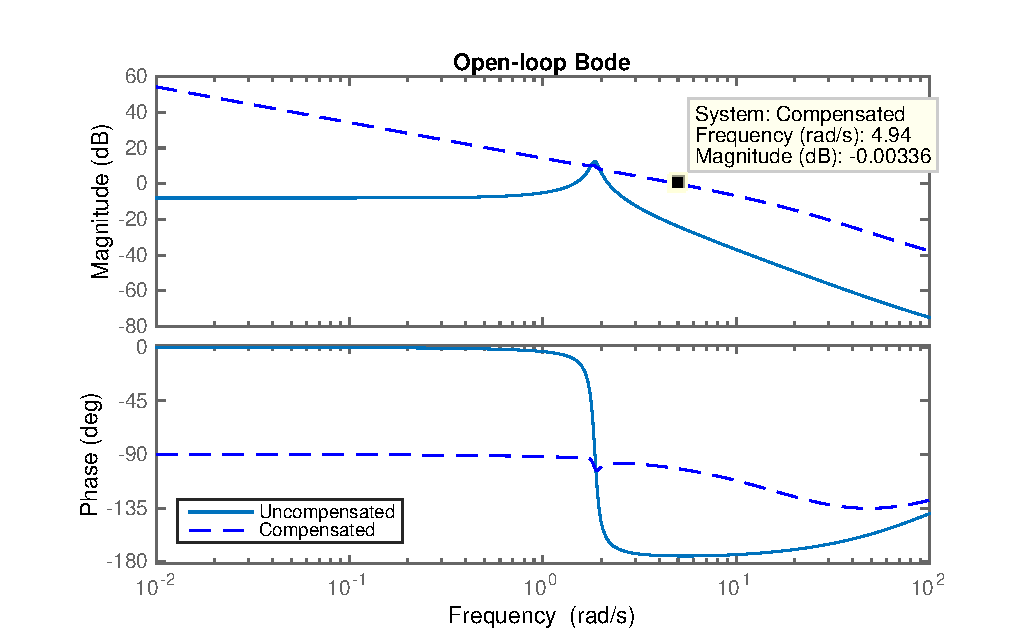
\includegraphics[height=.4\textheight]{figures/openloop_beta}
\caption{Open-loop Bode Plot for $\beta$ loop}
\end{center}
\end{figure}

\begin{figure}[h!]
\begin{center}
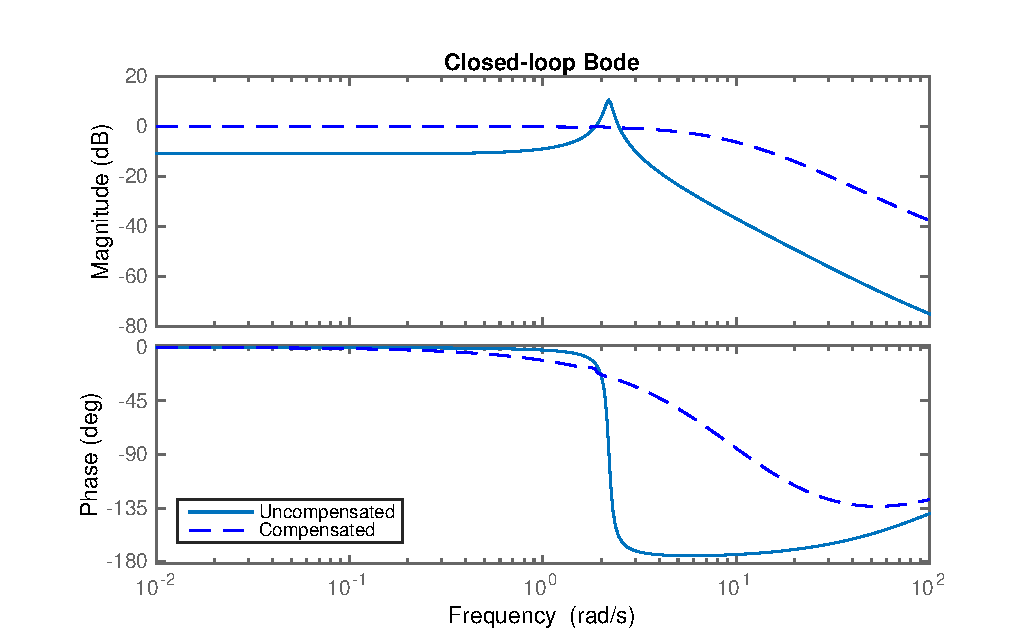
\includegraphics[height=.4\textheight]{figures/closeloop_beta}
\caption{Close-loop Bode Plot for $\beta$ loop}
\end{center}
\end{figure}

\clearpage
\section{Response to Command Inputs}
Two initial conditions were investigated (both commands were filtered with a filter of $\frac{25}{(s^2 + 10s + 25)}$):
\begin{enumerate}
\item a $\pm 5$ deg/sec doublet with each of the two pulses lasting 2 sec for the p-loop with no command for the $\beta$-loop
\item a $+ 5$ deg/sec command for the $\beta$-loop with no command for the $p$-loop\\
\end{enumerate}


\begin{figure}[h!]
\begin{center}
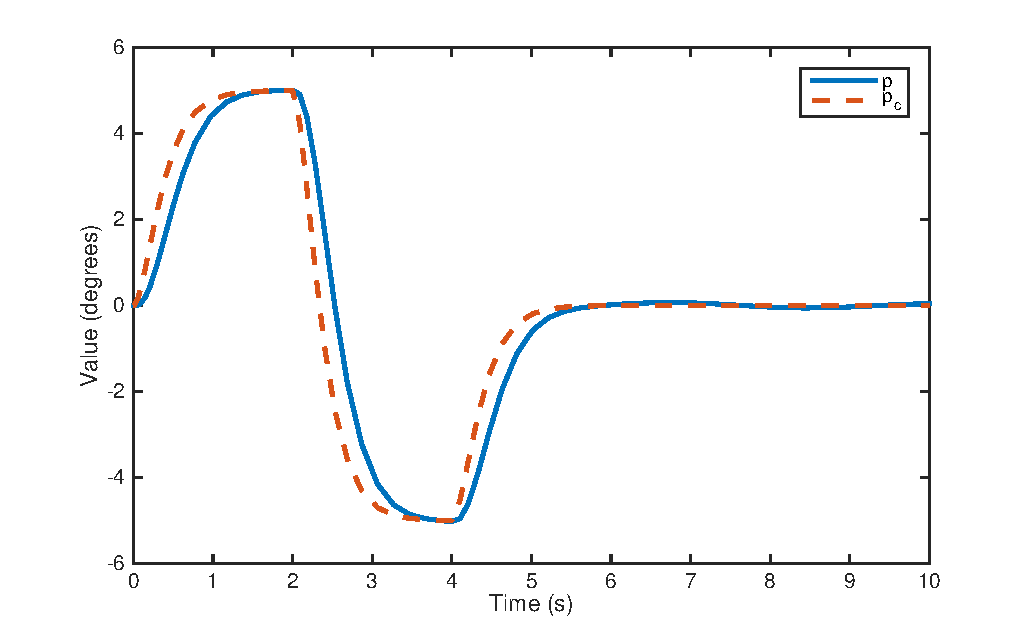
\includegraphics[height=.425\textheight]{figures/p2}
\caption{$p$ Response for Scenario 1}
\end{center}
\end{figure}

\begin{figure}[h!]
\begin{center}
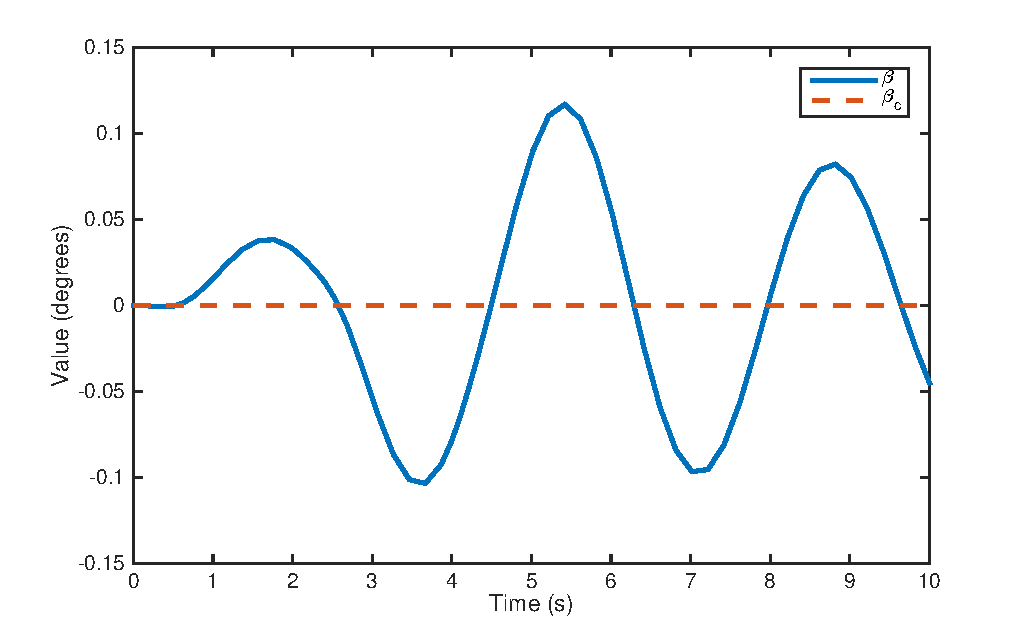
\includegraphics[height=.425\textheight]{figures/beta2}
\caption{$\beta$ Response for Scenario 1}
\end{center}
\end{figure}

\begin{figure}[h!]
\begin{center}
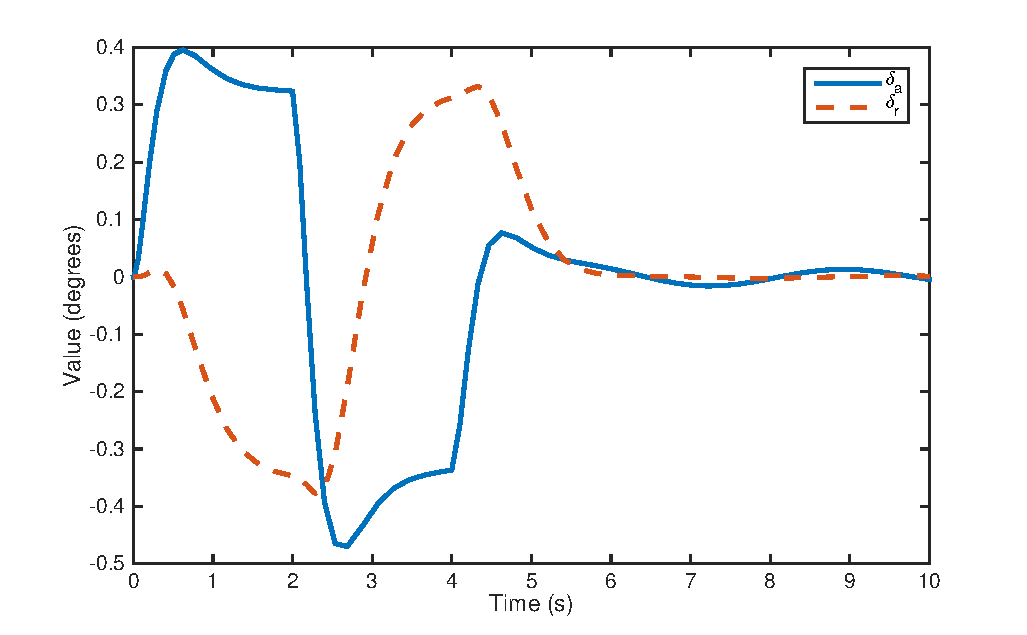
\includegraphics[height=.425\textheight]{figures/inputs2}
\caption{Command Inputs for Scenario 1}
\end{center}
\end{figure}

\begin{figure}[h!]
\begin{center}
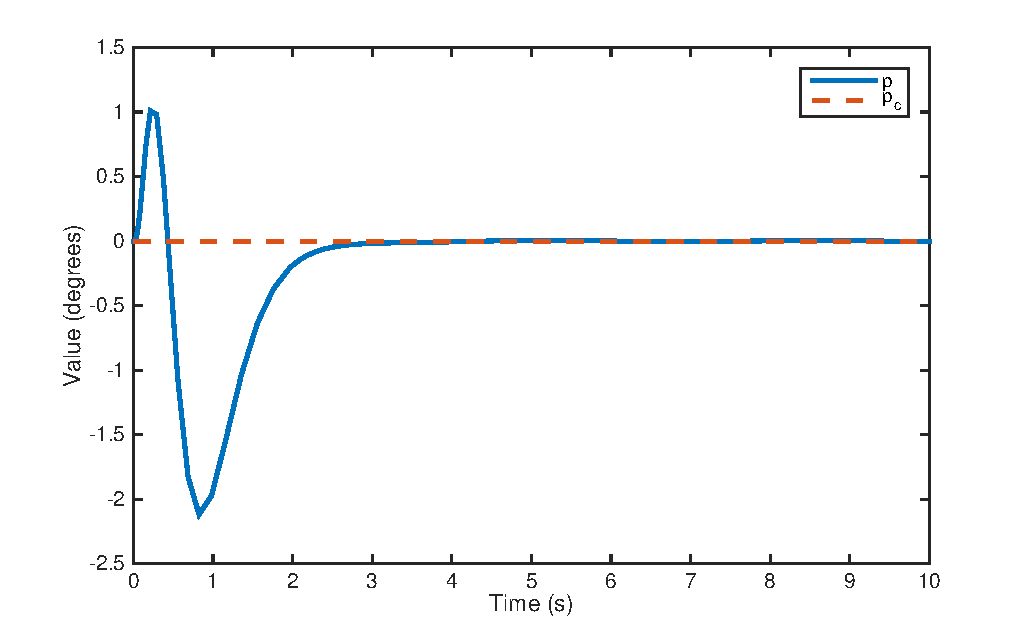
\includegraphics[height=.425\textheight]{figures/p1}
\caption{$p$ Response for Scenario 2}
\end{center}
\end{figure}

\begin{figure}[h!]
\begin{center}
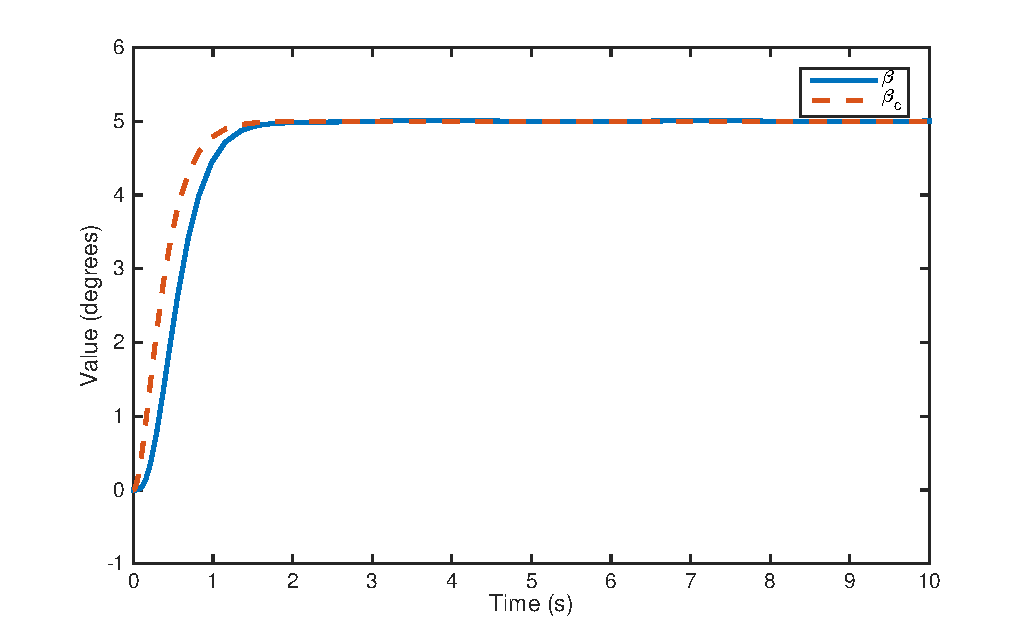
\includegraphics[height=.425\textheight]{figures/beta1}
\caption{$\beta$ Response for Scenario 2}
\end{center}
\end{figure}

\begin{figure}[h!]
\begin{center}
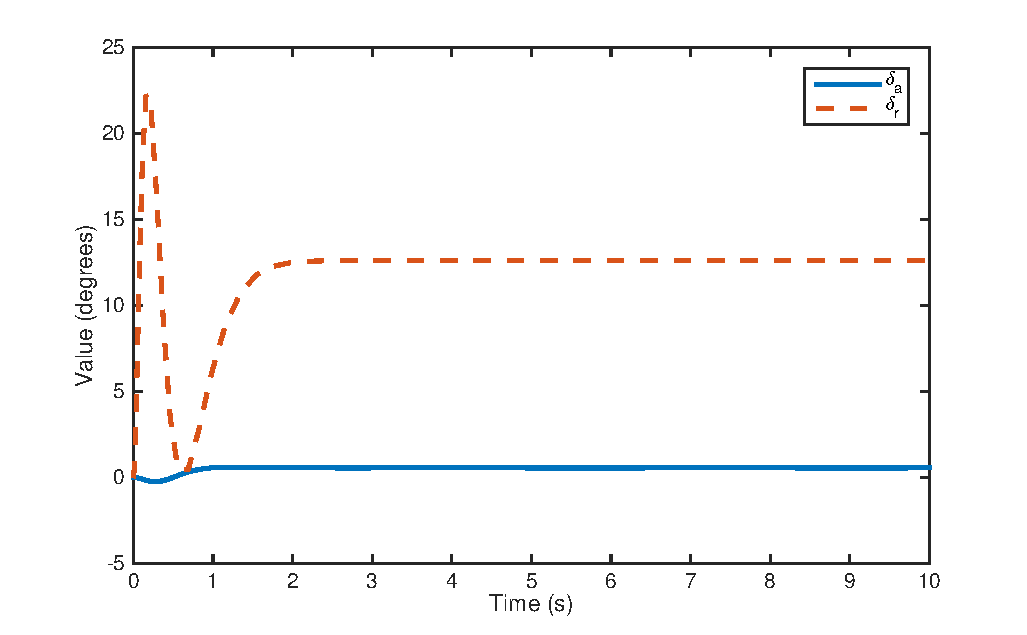
\includegraphics[height=.425\textheight]{figures/inputs1}
\caption{Command Inputs for Scenario 2}
\end{center}
\end{figure}


\end{document}
